\documentclass[%
11pt, english, parskip=false, headings=small,
headinclude=false, 
footinclude=false,oneside]{pst-doc}

\KOMAoptions{DIV=9}
\usepackage[latin1]{inputenc}
%
\usepackage{pst-func}
\usepackage{pst-optexp}
\let\verPstOptExp\fileversion
\let\datePstOptExp\filedate
\usepackage{pst-circ}
\usepackage{nicefrac}
\usepackage{longtable}
\usepackage{multicol}
\usepackage{multirow}
\usepackage{float}
\usepackage{prettyref}
\newrefformat{sec}{Sec.~\ref{#1}}
\lstset{%
  language=[LaTeX]TeX,
  texcsstyle = [20]\color{DOrange!60!black},
  moretexcs = [20]{lens, mirror, beamsplitter, optbox},
%  keywordstyle = [30]\color{green!30!black},
%  morekeywords = [30]{label},
  explpreset={pos=l,width=-99pt,overhang=0pt,hsep=5mm, varwidth,vsep=\bigskipamount,rframe={}},
  escapechar=�
}
%
% Addition from GL
%%%%%%%%%%%%%%%%%%%%%%%%%%%%%%%%%%%%%%%%%%%%%%%%%%%%%%%%%%%%%%%%%%%%%%%%%%%%%%%%%%%%%%%%%
\usepackage {etoolbox}
% \makeatletter
% \AtBeginEnvironment{LTXexample}{\let\lsthk@OutputBox\lsthk@OutputBox@H@@k\let\lstbasicfont\footnotesize}
% \AtBeginEnvironment{lstlisting}{\let\lsthk@OutputBox\lsthk@OutputBox@H@@k\let\lstbasicfont\footnotesize}
% %\AtBeginDocument{\preto\FV@VerbatimBegin{\let\lsthk@OutputBox\lsthk@OutputBox@H@@k\let\lstbasicfont\footnotesize}}
% %\AtBeginDocument{\preto\FV@VerbatimBegin{\let\lsthk@OutputBox\lsthk@OutputBox@H@@k\let\lstbasicfont\footnotesize}}
% \providerobustcmd*\ifrefundefined [1]{%
%   \begingroup%
%     \csname @safe@activestrue\endcsname%
%     \expandafter\endgroup\csname @\ifcsname r@#1\endcsname second\else first\fi oftwo\endcsname
% }% \ifrefundefined
% \def\lsthk@OutputBox@H@@k{%
%     \begingroup%
%       \let\lst@UM\@empty%
%       \edef\@tempc{sec:\detokenize\expandafter{\the\lst@token }}%\edef
%       \ifrefundefined{\@tempc}%
%     \endgroup%
%     \sethyperlistings%
% }% \lsthk@OutputBox@fcltxH@@k
% \def\sethyperlistings {\global\let \hyperlistingsreference =\@tempc
%      \endgroup \aftergroup \dohyperlistings }% after \hbox
% \def\dohyperlistings {\def\lst@alloverstyle ##1{\hyperlistings ##1}}
% \def\hyperlistings{%
%     \setbox\@tempboxa\hbox%
%     \bgroup%
%       \rlap{\hypersetup {linkcolor=.}\relax\fboxrule\z@%
%       \hyperref[\hyperlistingsreference]{\boxframe{\wd\@tempboxa}{\ht\@tempboxa}{\dp\@tempboxa}}}%
%       \unhbox\@tempboxa%
%     \egroup%
% }% \hyperlistings
% \let\lsthk@OutputBox\lsthk@OutputBox@H@@k
% \makeatother
% -----------------------------------------------------------
\newlength{\marglistwidth}
\newlength{\marglistsep}

\AtEndPreamble{%
  \deflength{\marglistwidth}{(\oddsidemargin+1in)*85/100}%
  \deflength{\marglistsep}{10pt}}

\newenvironment*{fieldlist}
  {\list{}{%
     \setlength{\labelwidth}{\marglistwidth}%
     \setlength{\labelsep}{\marglistsep}%
     \setlength{\leftmargin}{0pt}%
     \renewcommand*{\makelabel}[1]{\hss\color{sectioncolor}\marglistfont##1}}%
   \def\fielditem##1##2##3{%
     \item[##1]%
     \xLkeyword{##1}%
     \texttt{##2} \ifx##3\relax\else (default: \texttt{##3})\fi\par\nobreak
     \vspace{0.5\itemsep}}%
   \def\styleitem##1##2{%
     \item[##1]%
     \xLstyle{##1}\xLkeyword{addto##1}\xLkeyword{new##1}%
     \texttt{<psstyle>} \ifx##2\relax\else (default: \texttt{##2})\fi\par\nobreak
     \vspace{0.5\itemsep}}%
   \def\styleonlyitem##1##2{%
     \item[##1]%
     \xLstyle{##1}
     \texttt{<psstyle>} \ifx##2\relax\else (default: \texttt{##2})\fi\par\nobreak
     \vspace{0.5\itemsep}}}%
  {\endlist}
\newcommand*{\marglistfont}{\sffamily\small}

\newenvironment*{marglist}
  {\list{}{%
     \setlength{\labelwidth}{\marglistwidth}%
     \setlength{\labelsep}{\marglistsep}%
     \setlength{\leftmargin}{0pt}%
     \renewcommand*{\makelabel}[1]{\hss\marglistfont##1}}}
  {\endlist}
%
% New commands
%
\newcommand{\OptExpPackage}{\textsf{`pst-optexp'}}
\newcommand{\nodename}[1]{\emph{#1}}
\newcommand{\param}[1]{\normalfont\texttt{#1}}
\newcommand{\paramvalue}[1]{\texttt{#1}}
\newcommand{\defaultparam}[1]{\emph{default:} \paramvalue{#1}}
\newcommand{\paramitem}[3]{\item[\param{#1}:] \paramvalue{#2} (\defaultparam{#3})}
\newcommand{\styleitem}[2]{\item[\param{#1}:] \paramvalue{#2}}
\newcommand{\styleshape}[1]{\texttt{#1}}
\newcommand{\parampar}[1]{\marginpar{\Lkeyword{#1}}}
\newcommand{\stylepar}[1]{\paragraph{\Lstyle{#1}}\xLkeyword{addto#1}\xLkeyword{new#1}}

\newcommand{\nodedesc}[1]{\Largr{#1}}
\newcommand{\nodedescin}{\nodedesc{In}}%
\newcommand{\nodedescout}{\nodedesc{Out}}%

\def\Lstyle#1{\texttt{#1}\xLstyle{#1}}
\def\xLstyle#1{\index{#1@\texttt{#1}}\index{Style!#1@\texttt{#1}}}
\def\nxLstyle#1{\texttt{#1}}

\def\Ldipole#1{\nxLcs{#1}\xLdipole{#1}}
\def\xLdipole#1{\index{#1@\nxLcs{#1}}\index{Dipole object!#1@\nxLcs{#1}}}

\def\Ltripole#1{\nxLcs{#1}\xLtripole{#1}}
\def\xLtripole#1{\index{#1@\nxLcs{#1}}\index{Tripole object!#1@\nxLcs{#1}}}

\def\Lfdipole#1{\nxLcs{#1}\xLfdipole{#1}}
\def\xLfdipole#1{\index{#1@\nxLcs{#1}}\index{Fiber dipole object!#1@\nxLcs{#1}}}

\def\Lfmultipole#1{\nxLcs{#1}\xLmultipole{#1}}
\def\xLmultipole#1{\index{#1@\nxLcs{#1}}\index{Fiber multipole object!#1@\nxLcs{#1}}}

\newcommand{\dipoledesc}[1]{%
  \Ldipole{#1}\OptArgs%
  \nodedescin%
  \nodedescout%
  \Largb{label}%
}
\newcommand{\tripoledesc}[1]{%
  \Ltripole{#1}\OptArgs%
  \nodedescin%
  \nodedesc{center}%
  \nodedescout%
  \Largb{label}%
}

\newcommand{\fiberdipoledesc}[1]{%
  \Lfdipole{#1}\OptArgs%
  \nodedescin%
  \nodedescout%
  \Largb{label}%
}

\newcommand{\fibermultipoledesc}[1]{%
  \Lfmultipole{#1}\OptArgs%
  \nodedescin%
  \nodedescout%
  \Largb{label}%
}

\newcolumntype{T}{>{\ttfamily}l}
\newcolumntype{B}{>{\bfseries}l}
\newcommand{\refstringexplanation}[0]{%
  A \paramvalue{<ref string>} is any combination of \paramvalue{c}
  (center), \paramvalue{t} (top), \paramvalue{b} (bottom), \paramvalue{l}
  (left), \paramvalue{r} (right)}

\makeatletter
\renewenvironment{description}
  {\list{}{\labelwidth\z@ \itemindent-0.5\leftmargin
    \itemsep0pt \parsep0pt
    \let\makelabel\descriptionlabel}}
  {\endlist}
\makeatother

\psset{usefiberstyle=true}
\addtopsstyle{Fiber}{linecolor=red,linewidth=1.5\pslinewidth}
\addtopsstyle{Beam}{linewidth=1.5\pslinewidth}

\makeatletter
\renewcommand\maketitle{%
\thispagestyle{empty}%
\begin{titlepage}
\begin{pspicture}(1.6in,0.685in)(10,21.7)
  \psframe[fillstyle=solid,linecolor=lightgray,fillcolor=lightgray,linestyle=solid](0,-5.75)(21.5,10)
  \psframe[fillstyle=solid,linecolor=Orange!85!Red,fillcolor=Orange!85!Red,linestyle=solid](0,10)(21.5,10.5)
  \psframe[fillstyle=solid,linecolor=Orange!85!Red,fillcolor=Orange!85!Red,linestyle=solid](0,21.1)(21.5,21.2)
  \rput[lb](3,22){\Huge\sffamily\color{Orange!65!Red}\psscalebox{2}{\textbf{PSTricks}}}
  \rput[lb](3,14.1){\parbox{15cm}{\sffamily\RaggedRight\bfseries\huge\@title}}
  \rput[lb](3,12.6){\parbox{13cm}{\sffamily\Large\@subtitle}}
  \rput[lb](3,7.6){\parbox{13cm}{\sffamily\@date}}
  \rput[lb](3,-2.6){\parbox[b]{17cm}{\sffamily\RaggedRight 
    \ifx\@docauthor\empty~\else Documentation by\fi\hfill\makebox[7cm][l]{Package author(s):}\\
    \ifx\@docauthor\empty~\else{\bfseries\tabular[t]{@{}l@{}}\@docauthor\endtabular}\fi\hfill\makebox[7cm][l]{%
      \bfseries\tabular[t]{@{}l@{}}\@author\endtabular}}}
 \rput[C](11,4){\bgImage}%
\end{pspicture}%
\end{titlepage}}
\makeatother

%%%%%%%%%%%%%%%%%%%%%%%%%%%%%%%%%%%%%%%%%%%%%%%%%%%%%%%%%%%%%%%%%%%%%%%%
 \title{\texttt{pst-optexp}\\ A PSTricks package to draw optical experimental setups\\ \small v.\verPstOptExp}
 \author{Christoph Bersch}
 \date{\datePstOptExp}
\def\bgImage{\psset{unit=1.3}
\begin{pspicture}[showgrid=false](-0.2,0.1)(8.2,5.3)
  \pnode(0,3){M1}
  \pnode(8,3){M2}
  \pnode(8,0.5){In}
  \pnode(6.5,0.5){Min}
  \pnode(6.5,3){Pin}
  \pnode(4.5,3){Min2}
  \pnode(1.5, 0.5){Mout}
  \pnode(1.5,3){Pout}
  \pnode(3.5,3){Mout2}
  \pnode(0,0.5){Out}
  \definecolor[ps]{bl}{rgb}{tx@addDict begin Red Green Blue end}%
  \addtopsstyle{Beam}{linecolor=bl, linejoin=1}
  \psset{mirrortype=extended, mirrordepth=0.15}
  \newpsstyle{ExtendedMirror}{linestyle=none, hatchwidth=0.5\pslinewidth, hatchsep=1.2\pslinewidth,%
                fillstyle=hlines}%
  \begin{optexp}
  \mirror[mirrorwidth=4, mirrorradius=10.4](M2)(M1)(M2){}
  \mirror[mirrorwidth=4, mirrorradius=10.4](M1)(M2)(M1){}
  \mirror(In)(Min)(Pin){}
  \optprism[n=1.85, addtoOptComp={linewidth=1.5\pslinewidth}](Min)(Pin)(Min2){}
  \mirror[compshift=0.4](Pin)(Min2)(Pin){}
  \mirror[compshift=-0.4](Pout)(Mout2)(Pout){}
  \optprism[n=1.85, compshift=0.15, linewidth=1.5\pslinewidth](Mout2)(Pout)(Mout){}
  \mirror(Pout)(Mout)(Out){}
  \multido{\i=0+1}{40}{%
    \pstVerb{%
      \i\space 650 400 sub 39 div mul 400 add 
      tx@addDict begin wavelengthToRGB end }%
    \drawbeam[nadd=-0.002 \i\space mul]{(In)}{3}{4}{5}{2}{1}{6}{7}{8}{(Out)}
  }%
  \newpsstyle{Beam}{linecolor=red}
  \bglayer{%
    \psline[style=Beam,ArrowInside=->, linewidth=2\pslinewidth, arrowinset=0](In)(\OENodeIn{@3})(\OENodeOut{@4})
  }
  \drawbeam[startvec=0.005,startpos=0.1, addtoBeam={arrows=<-, linewidth=2\pslinewidth, arrowinset=0}]{([Xnodesep=-0.2]Out)}{8}{7}
\end{optexp}
\rput(4,4.5){%
  \psframe[fillstyle=solid,fillcolor=gray!70](-0.1, -0.6)(0.1, 0.7)
  \multido{\r=-0.5+0.1}{12}{%
    \psline[linewidth=0.5\pslinewidth](-0.1,\r)(0.1,\r)
  }%
}%
\end{pspicture}}
\begin{document}
\maketitle

\clearpage
\tableofcontents
\clearpage

\section{Introduction}
The package \LPack{pst-optexp} is a collection of optical components
that facilitate easy sketching of optical experimental
setups. Mechanisms for proper alignment of different components are
provided internally. This way the user does not have to care for proper
orientation of the elements. Macros for convenient definition of new 
user-defined components are also provided.

\section{Backward compatibility}

\begin{fieldlist}
\fielditem{namingscheme}{old|new}{new}
Version 3.0 introduced a lot of advanced features which made it too difficult to
maintain full backward compatibility with version 2.x. However, using the
\Loption{compat} package option allows you to compile old setups but without
profiting from the new features. If you only need the old naming scheme, because
you accessed internal nodes directly, then you must only set
\Lkeyword{oldnamingscheme}.
\end{fieldlist}


\section{Concept and General Behavior}\label{sec:general}

This section introduces into the basic concepts of the package design and
explains the parameters and commands which are supported by most optical
objects.

\subsection{Concept}

The objects provided by \LPack{pst-optexp} can be differentiated into
two different categories: free-ray and fiber-optical objects.

The free-ray units are subdivided in two different kinds: dipoles which
require two reference points for alignment and do not alter the
direction of passing light beams (e.g. lenses and retardation plates)
and tripoles which work in reflection and require three reference points
(mirrors, gratings, beamsplitters etc.).

For free-ray setups one usually has a few straight light paths in which
several different objects are to be arranged. In this case it is very
convenient to define only two nodes for each light path. The objects are
placed on this light path using the different positioning parameters
(see \prettyref{sec:positioning}) of the package. After having arranged
everything, the beams themselves are drawn (see \prettyref{sec:connecting}).

The fiber-optical objects can be classified as dipoles, tripoles and quadrupoles
which have a corresponding number of fiber connections. Their handling differs
in some aspects from the free-ray objects. The fiber optics are directly
connected to the reference nodes. Every input and output fiber can be flexibly
customized for each object (see \prettyref{sec:styles}). Positioning of the
fiber dipoles is handled equivalently to the free-ray dipoles. Tripoles and
quadrupoles can be found only as different coupler types. Their positioning
mechanisms are a bit more involved and explained in the respective section
(\prettyref{sec:coupler}).

Some hybrid dipoles (optbox, detector etc.) can be used both as
fiber-optical or free-ray elements. 

\subsection{General Settings}

\begin{description}
\paramitem{angle}{<degree>}{0}
\paramitem{compshift}{<num>}{0}
\paramitem{optional}{<boolean>}{false}
\styleitem{OptionalStyle}{<psstyle>}{}
\paramitem{showoptdots}{<boolean>}{false}
\end{description}

Some generic parameters which can be used for all objects.

\begin{fieldlist}
\fielditem{angle}{<num>}{0}

Rotate an object by \nxLkeyword{angle} degrees.

\fielditem{optional}{<boolean>}{false}
\styleonlyitem{OptionalStyle}{linestyle=dashed, dash=1.5pt 1pt}

Can be used with every object and marks it as optional. The style of an
optional element can be configured by changing the psstyle
\nxLkeyword{OptionalStyle}.

\begin{LTXexample}
\begin{pspicture}(3,1.5)
\lens[optional, beam](0,1)(3,1){L}
\end{pspicture}
\end{LTXexample}

\fielditem{showoptdots}{<boolean>}{false}

Draw some internal nodes which are used to place the object and the
label. The black points are used for positioning, the red points mark
the label references.
\medskip

\begin{LTXexample}
\begin{pspicture}(3,2)
\mirror[showoptdots,
          beam](0,1)(1.9,1)(1.9,0){mirror}
\end{pspicture}
\end{LTXexample}
\end{fieldlist}

\subsection{Using PSStyles}\label{sec:styles}

The appearance of many functional parts of \LPack{pst-optexp} objects is
controlled via psstyles. These are collections of parameters which are
applied only to selected subparts of the objects. In general, these
psstyles can be overwritten with the \Lcs{newpsstyle} macro and extended
with the \Lcs{addtopsstyle} macro.

\begin{fieldlist}
\styleitem{OptComp}{}
Affects only the appearence of the optical
components. This was introduced, because using only the standard
graphics parameters changes also the connections that are drawn within
the component.

\medskip

\begin{LTXexample}
\begin{pspicture}(3,4)
  \psset{beam}
  % wrong, also beam width is changed
  \mirror[linewidth=3\pslinewidth]%
         (0,3)(2,3)(2,2){mirror}
  % correct result
  \mirror[addtoOptComp={linewidth=3\pslinewidth}]%
         (0,1)(2,1)(2,0){mirror}
\end{pspicture}
\end{LTXexample}

\styleitem{OptionalStyle}{style=OptComp, linestyle=dashed, dash=1.5pt 1pt}
\end{fieldlist}

\subsection{Positioning}\label{sec:positioning}
\begin{fieldlist}
\fielditem{position}{<num>}{}

Equivalent to the \Lkeyword{npos} parameter of \Lcs{ncput} (can be any number
from 0 to 1) and controls the relative position of object between the two
reference points. It is only not available for the free-ray tripoles.

\medskip

\begin{LTXexample}
\begin{pspicture}(3,1.5) 
  \lens[beam, position=0.8](0,1)(3,1){L}
\end{pspicture}
\end{LTXexample}

\fielditem{abspos}{<num>}{}
The parameter \Lkeyword{abspos} allows absolute positioning between the
two reference nodes. Its value is given in psunits.

\medskip

\begin{LTXexample}
\begin{pspicture}(3,1.5) 
  \lens[beam, abspos=1](0,1)(3,1){L}
\end{pspicture}
\end{LTXexample}

\fielditem{compshift}{<num>}{0}

\begin{LTXexample}
\begin{pspicture}(3,2) 
  \lens[compshift=0.1, n=1](0,1)(3,1){L}
  \addtopsstyle{Beam}{startvecabs, startvec=1 0}
  \drawbeam{(0,1)}{}{(3,1)}
\end{pspicture}
\end{LTXexample}

\bigskip

\begin{LTXexample}
\begin{pspicture}(3,2) 
  \mirror[beam, compshift=0.2, startvecabs, startvec=1 0, labelangle=45](0,1)(2,1)(2,0){mirror}
\end{pspicture}
\end{LTXexample}

\end{fieldlist}


\subsection{Labels}\label{sec:labels}

\begin{fieldlist}
\fielditem{labeloffset}{<num>}{0.8}

Specify the offset from the label reference node of the object which in most
cases is the center.

\fielditem{labelstyle}{<macro>}{\nxLcs{small}}

Define the textstyle that is used to typeset the label. 

\fielditem{labelalign}{<ref string>}{c}

Has the same meaning as the refpoint of \Lcs{rput} and can take the same values.

\fielditem{labelangle}{<num>}{0}

Set the label rotation angle around the
object. \Lkeyword{labelref} can be used to change the reference system.

\fielditem{labelref}{relative|relgrav|global}{relgrav}

Set the reference coordinate system for the \Lkeyword{labelangle} and the orientation of
the label text. The detailed behaviour is best illustrated looking at
the following three examples.

\medskip

\begin{LTXexample}
\begin{pspicture}(-2,-2)(2.5,2)
  \psset{endbox, optboxwidth=1, optboxheight=0.6}
  \multido{\i=0+45}{8}{%
    \optbox[labelref=relative,
            labeloffset=0](0,0)(1;\i){\i}
  }
\end{pspicture}
\end{LTXexample}

\bigskip

\begin{LTXexample}
\begin{pspicture}(-2,-2)(2.5,2)
  \psset{endbox, optboxwidth=1, optboxheight=0.6}
  \multido{\i=0+72}{5}{%
    \optbox[labelref=relgrav](0,0)(1;\i){\i}
  }
\end{pspicture}
\end{LTXexample}

\bigskip

\begin{LTXexample}
\begin{pspicture}(-2,-2)(2.5,2)
  \psset{endbox, optboxwidth=1, optboxheight=0.6}
  \multido{\i=0+72}{5}{%
    \optbox[labelref=global](0,0)(1;\i){\i}
  }
\end{pspicture}
\end{LTXexample}

\medskip

\fielditem{label}{<offset>[ <angle>[ <ref string>[ <labelref>]]]}{}

Allows simplified notation for changing more than one
label-related parameter. It takes up to four space-separated arguments
(\nxLkeyword{labeloffset}, \nxLkeyword{labelangle}, \nxLkeyword{labelalign}, and
\nxLkeyword{labelref}). Unchanged arguments may be specified with a dot.

\medskip

\begin{LTXexample}
\begin{pspicture}(0,0)(4,3)
  \psset{endbox, beam}
  \optbox[label=0.7](1.5,2.5)(2.5,2.5){label}
  \optbox[label=1 -45](1.5,1)(2.5,1){$-45$}
  \optbox[label=0 . . relative]%
         (0.6,0.6)(0.6,1.6){relative}
\end{pspicture}
\end{LTXexample}

\end{fieldlist}

\subsection{Named Objects}\label{sec:namedobj}

\begin{fieldlist}
\fielditem{compname}{<string>}{}
Every \LPack{pst-optexp} object of an experimental setup can
be assigned a name that is unique within one pspicture environment. The
name is defined with the parameter \Lkeyword{compname} which is
defineable only directly within a \LPack{pst-optexp} object.

\medskip

\begin{lstlisting}
\optbox[compname=MyBox](A)(B){Box} % valid use of 'compname'
\psset{compname=MyName}            % not valid, gives an error
\end{lstlisting}
\end{fieldlist}
\medskip

\subsection{Nodes For External Usage}\label{sec:extnode}

Some of the objects can provide a supplementary node for additional
connections. A laser diode may be connected for example to a frequency synthesizer
(use package \LPack{pst-circ}) or a detector to a computer.

\begin{fieldlist}
\fielditem{extnode}{<refstring>}{}

Controls the position of the additional node and
takes a \paramvalue{<ref string>} as its argument. By default this
parameter is empty (\paramvalue{\{\}}) and no node is created.

The name of the new node depends on the \Lkeyword{compname} parameter
(see Sec.~\ref{sec:namedobj} for naming conventions). If \nxLkeyword{compname} is empty
the new node is named \nodename{ExtNode} by default and overwritten by
following objects.

Table.~\ref{tab:nodes} shows all objects which provide an external
node. Some allow any possible \paramvalue{<ref string>} for \Lkeyword{extnode}, others have
only one reasonable possibility (e.g. piezo mirror, see
Sec.~\ref{sec:mirror}) which does not depend on the actual value of \Lkeyword{extnode}.

\bigskip

\begin{LTXexample}[pos=t, vsep=8mm]
\begin{pspicture}[showgrid=true](11,3) 
   \psset{beam, beamInside=false, labelangle=-90, labeloffset=0.3}
   \optbox[extnode=tl](0,2.5)(3,2.5){\texttt{tl}}\psdot(\OENodeExt{})
   \optbox[extnode=l](0,1.5)(3,1.5){\texttt{l}}\psdot(\OENodeExt{})
   \optbox[extnode=bl](0,0.5)(3,0.5){\texttt{bl}}\psdot(\OENodeExt{})
   \optbox[extnode=t](4,2.5)(7,2.5){\texttt{t}}\psdot(\OENodeExt{})
   \optbox[extnode=c](4,1.5)(7,1.5){\texttt{c}}\psdot(\OENodeExt{})
   \optbox[extnode=b](4,0.5)(7,0.5){\texttt{b}}\psdot(\OENodeExt{})
   \optbox[extnode=tr](8,2.5)(11,2.5){\texttt{tr}}\psdot(\OENodeExt{})
   \optbox[extnode=r](8,1.5)(11,1.5){\texttt{r}}\psdot(\OENodeExt{})
   \optbox[extnode=br](8,0.5)(11,0.5){\texttt{br}}\psdot(\OENodeExt{})
\end{pspicture}
\end{LTXexample}

\begin{table}[H]
\centering
  \begin{tabular}{llc}
    \toprule
    Object & possible extnode positions &\\
    \midrule
    %
    \Lcs{optbox} & 
    all (any combination of \paramvalue{t}, \paramvalue{r}, \paramvalue{l} and \paramvalue{b}) &
    \begin{pspicture}[shift=-0.3](0,-0.4)(1,0.4)
       \psframe(0,-0.25)(1,0.25)
       \psdot(0,-0.25)\psdot(0.5,-0.25)\psdot(1,-0.25)
       \psdot(0,0)\psdot(0.5,0)\psdot(1,0)
       \psdot(0,0.25)\psdot(0.5,0.25)\psdot(1,0.25)
    \end{pspicture}\\
    %
    \Lcs{mirror} & 
    one fixed position (only for \Lkeyword{mirrortype=piezo}) &
    \begin{pspicture}[shift=-0.3](1,0.8)
       \mirror[mirrortype=piezo,extnode=t](0,0.4)(0.5,0.4)(0.5,0){}\psdot(ExtNode)
    \end{pspicture}\\
    %
    \Lcs{optdetector} & 
    one (for \Lkeyword{dettype=round}) &
    \begin{pspicture}[shift=-0.3](1,0.8)
       \optdetector[detsize=0.6, extnode=r](0,0.4)(0.5,0.4){}
       \psdot(ExtNode)
    \end{pspicture}\\
    %
    & all (for \Lkeyword{dettype=diode})& see \Lcs{optbox}\\
    \Lcs{optmzm} & all& see \Lcs{optbox}\\
    \Lcs{optfilter} & all & see \Lcs{optbox}\\
    \Lcs{optswitch} & all & see \Lcs{optbox}\\
    \Lcs{fiberdelayline} & all & see \Lcs{optbox}\\
    \bottomrule
  \end{tabular}
  \caption{The objects which may provide an external node when parameter
    \Lkeyword{extnode} is not empty. Some allow different positions of the
    node and for some only a fixed node makes sense.}\label{tab:nodes}
\end{table}
\end{fieldlist}

\newpage

\section{Free-Ray Objects}

The general appearance of all objects can be customized using the
standard PSTricks parameter like \Lkeyword{linewidth}
or \Lkeyword{fillstyle}. Some components allow changing a special part
(e.g. for a piezo mirror) for which they use certain psstyles. For the
automatic beam connections the \styleshape{Beam} style is used.

\subsection{Lens}\label{sec:lens}

\begin{BDef}
\dipoledesc{lens}
\end{BDef}

\begin{fieldlist}
\fielditem{lensheight}{<num>}{1}
\fielditem{lensradius}{<num> [<num>]}{\{\}}
\fielditem{lensradiusleft}{<num>}{1}
\fielditem{lensradiusright}{<num>}{1}
\fielditem{lens}{<num> [<num> [<num> [<num>]]]}{\{\}}

\begin{LTXexample}[width=5.5cm]
\begin{pspicture}[showgrid=true](5,6)
  % concave lenses
  \pnode(0,5){A}\pnode(5,5){B}
  \psline[style=Beam](A)(B)
  \lens[position=0.2](A)(B){L}
  \lens[lensradius=-1,position=0.5](A)(B){L}
  \lens[lens=-1.5 1,position=0.7](A)(B){L}
  % convex lenses
  \pnode(0,3){A}\pnode(5,3){B}
  \psline[style=Beam](A)(B)
  \lens[position=0.2,lens=1 -1](A)(B){L}
  \lens[lens=0 -1](A)(B){L}
  \lens[lens=1 0,position=0.7](A)(B){L}
\end{pspicture}
\end{LTXexample}

\fielditem{thicklens}{<boolean>}{false}
\fielditem{lenswidth}{<num>}{0.2}

\begin{LTXexample}[width=5cm]
\begin{pspicture}(5,2)
  % thick lenses
  \pnode(0,1){A}\pnode(5,1){B}
  \psline[style=Beam](A)(B)
  \lens[position=0.3, lens=-1.5 1 1 0.5, thicklens](A)(B){thicklens}
  \lens[lens=0 -1, position=0.7, fillstyle=solid, fillcolor=blue!30!white](A)(B){lens}
\end{pspicture}
\end{LTXexample}

\end{fieldlist}

\medskip

The shape of a lens is defined by its two surface radii. A negative
radius gives a concave, a positive radius a convex and a radius of
\texttt{0} a plain surface. The parameters \Lkeyword{lensradiusleft}
and \Lkeyword{lensradiusright} allow to define independent values for
both surfaces. \Lkeyword{lensradius} sets both curvatures to the same
value. Usually only \Lkeyword{lensheight} and the two radii are used to
construct the lens. The thickness (or width) is determined
automatically. Manually controlling the thickness of the lens can be
achived by setting \Lkeyword{thicklens}
to \paramvalue{true}. Then \Lkeyword{lenswidth} is used as width of the
lens at its waist. Finally, the parameter \Lkeyword{lens} allows the
definition of all relevant lens parameters at once. It consists of one
up to four space-separated numbers. The first one gives the left
radius. If no further value is set, the right radius will be set to the
same value and all other parameters are left unchanged. Using two
numbers defines two different radii. The third optional value defines
the \Lkeyword{lensheight} and the fourth one the \Lkeyword{lenswidth}
which is use only if \Lkeyword{thicklens} is set to \Lkeyword{true}.

\medskip
\subsection{Optical Plate}

\begin{BDef}
\dipoledesc{optplate}
\end{BDef}

\begin{fieldlist}
\fielditem{plateheight}{<num>}{1}
\fielditem{platelinewidth}{<num>}{2\nxLcs{pslinewidth}}

\begin{LTXexample}[width=3cm]
\begin{pspicture}(3,1.5)
  \optplate[beam](0,1)(3,1){filter}
\end{pspicture}
\end{LTXexample}

\fielditem{angle}{<degree>}{0}

\begin{LTXexample}[width=3cm]
\begin{pspicture}(3,1.5)
  \optplate[angle=10, beam](0,1.2)(3,1.2){glass plate}
\end{pspicture}
\end{LTXexample}

\end{fieldlist}

\subsection{Retardation Plate}

\begin{BDef}
\dipoledesc{optretplate}
\end{BDef}

\begin{fieldlist}
\fielditem{plateheight}{<num>}{1}
\fielditem{platewidth}{<num>}{0.1}

\begin{LTXexample}[width=3cm]
\begin{pspicture}(3,1.5)
  \pnode(0,1){A}
  \pnode(3,1){B}
  \optretplate[beam](A)(B){$\nicefrac{\lambda}{2}$}
\end{pspicture}
\end{LTXexample}
\end{fieldlist}

\subsection{Pinhole}

\begin{BDef}
\dipoledesc{pinhole}
\end{BDef}

\begin{fieldlist}
\fielditem{outerheight}{<num>}{1}
\fielditem{innerheight}{<num>}{0.1}
\fielditem{phlinewidth}{<num>}{2\nxLcs{pslinewidth}}

\begin{LTXexample}[width=3cm]
\begin{pspicture}(3,1.5)
  \pnode(0,1){A}
  \pnode(3,1){B}
  \pinhole[beam](A)(B){PH}
\end{pspicture}
\end{LTXexample}
\end{fieldlist}

\subsection{Crystal}\label{sec:crystal}

\begin{BDef}
\dipoledesc{crystal}
\end{BDef}

\begin{description}
\paramitem{crystalwidth}{<num>}{1.4}
\paramitem{crystalheight}{<num>}{0.6}
\paramitem{caxislength}{<num>}{0.6}
\paramitem{caxisinv}{<boolean>}{false}
\paramitem{voltage}{<boolean>}{false}
\paramitem{lamp}{<boolean>}{false}
\paramitem{lampscale}{<num>}{0.3}
\paramitem{angle}{<degree>}{0}
\paramitem{rotateref}{<ref string>}{c}
\end{description}

\noindent For a discussion of the \Lkeyword{angle} and \Lkeyword{rotateref}
parameters see Sec.~\ref{sec:box} about boxes.  \medskip

\begin{LTXexample}[width=3.5cm]
\begin{pspicture}[showgrid=true](3,2)
  \pnode(0,1.2){A}
  \pnode(3,1.2){B}
  \crystal[fillstyle=solid, fillcolor=yellow!90!black, labelangle=-45, labeloffset=1.2, voltage, lamp, beam](A)(B){SBN:Ce}
\end{pspicture}
\end{LTXexample}

\medskip

\subsection{Box}\label{sec:box}

\begin{BDef}
\dipoledesc{optbox}
\end{BDef}

\begin{fieldlist}
\fielditem{optboxheight}{<num>}{0.8}
\fielditem{optboxwidth}{<num>}{1.4}

\begin{LTXexample}[width=3cm]
\begin{pspicture}(3,2)
  \optbox[beam](0,0)(3,2){box}
\end{pspicture}
\end{LTXexample}

\fielditem{endbox}{<boolean>}{false}

\begin{LTXexample}[width=3cm]
\begin{pspicture}(3,2)
  \optbox[beam, endbox](0,0)(1.5,1){box}
\end{pspicture}
\end{LTXexample}

\bigskip

\begin{LTXexample}[width=3cm]
\begin{pspicture}(3,2)
  \pnode(0,0){A}\pnode(1.5,1){B}
  \optbox[beam, endbox, label=0 . . relative](A)(B){box}
\end{pspicture}
\end{LTXexample}

\fielditem{angle}{<degree>}{0}
\fielditem{rotateref}{<ref string>\footnote{\refstringexplanation}}{c}

The parameter \Lkeyword{angle} describes the tilt of the box
relative to the reference line defined by the two reference nodes. The
reference point for the rotation can be defined
with \Lkeyword{rotateref} which can take any combination
of \paramvalue{c}, \paramvalue{t}, \paramvalue{b}, \paramvalue{l}
and \paramvalue{r} (compare with \Lkeyword{extnode} in
Sec.~\ref{sec:extnode}). Note, that all connection-related nodes are
also rotate, while the label is not affected.

\medskip

\begin{LTXexample}[width=3cm]
\begin{pspicture}(3,2)
  \optbox[angle=20, beam, rotateref=l, labeloffset=0.5](0,1)(3,1){box}
\end{pspicture}
\end{LTXexample}

\fielditem{refractiveindex}{<num>}{\{\}}

Together with the parameter \Lkeyword{refractiveindex} this
can be exploited to sketch the refraction through a tilted homogeneous
medium (e.g. a glass plate). Then, however, the reference nodes for the
beam connection must be corrected which is rather easy using the outer
nodes of the object as coordinate references and the \texttt{|} node
operator.

\medskip

\begin{LTXexample}[width=3cm]
\begin{pspicture}(3,1.5)
  \pnode(0,1){A}\pnode(3,1){B}
  \optbox[labeloffset=0.8, optboxwidth=0.5, optboxheight=1, angle=20, n=2.3, compname=Box](A)(B){glass plate}
  \drawbeam{(A|\OENodeIn{Box})}{Box}
  \drawbeam{Box}{(B|\OENodeOut{Box})}
\end{pspicture}
\end{LTXexample}
\end{fieldlist}

\subsection{Detector}

\begin{BDef}
\dipoledesc{optdetector}
\end{BDef}

\begin{fieldlist}
\fielditem{detsize}{<num>}{0.8}

\begin{LTXexample}[width=3cm]
\begin{pspicture}(3,2)
  \pnode(0,0){A}\pnode(1.5,1){B}
  \optdetector[beam](A)(B){detector}
\end{pspicture}
\end{LTXexample}

\fielditem{dettype}{round|diode}{round}

\begin{LTXexample}[width=3cm]
\begin{pspicture}(3,2)
  \pnode(0,0){A}\pnode(1.5,1){B}
  \optdetector[beam, dettype=diode](A)(B){detector}
\end{pspicture}
\end{LTXexample}
\end{fieldlist}

\subsection{Optical Diode}\label{sec:optdiode}


\begin{BDef}
\dipoledesc{optdiode}
\end{BDef}

\begin{fieldlist}
\fielditem{optdiodesize}{<num>}{0.8}

\begin{LTXexample}[varwidth]
\begin{pspicture}(3,2)
   \optdiode[beam, beamInside=false](0,1)(3,1){Diode}
\end{pspicture}
\end{LTXexample}
\end{fieldlist}

\subsection{Dove Prism}\label{sec:doveprism}

\begin{BDef}
\dipoledesc{doveprism}
\end{BDef}

\begin{description}
  \paramitem{doveprismsize}{<num>}{0.6}
\end{description}

\medskip

\begin{LTXexample}[width=3.5cm]
\begin{pspicture}[showgrid=true](3,2)
  \doveprism[beam](0,1)(3,1){Dove}
\end{pspicture}
\end{LTXexample}
\medskip

\subsection{Polarization}

\begin{BDef}
\Lcs{polarization}\OptArgs\coord{\text{in}}\coord{\text{out}}
\end{BDef}

\begin{description}
\paramitem{poltype}{parallel|perp|misc|lcirc|rcirc}{parallel}
\paramitem{polsize}{<num>}{0.6}
\paramitem{pollinewidth}{<num>}{0.7\nxLcs{pslinewidth}}
\end{description}

\medskip

\begin{LTXexample}[width=3.4cm]
\begin{pspicture}[showgrid=true](3,5)
  \pnode(0,0.5){A1}\pnode(3,0.5){B1}\pnode(0,1.5){A2}
  \pnode(3,1.5){B2}\pnode(0,2.5){A3}\pnode(3,2.5){B3}
  \pnode(0,3.5){A4}\pnode(3,3.5){B4}\pnode(0,4.5){A5}
  \pnode(3,4.5){B5}\psset{style=Beam}
  \multido{\i=1+1}{5}{\psline(A\i)(B\i)}
  \psset{linecolor=black}
  \polarization[poltype=misc,position=0.2](A5)(B5)
  \polarization[poltype=perp,position=0.35](A4)(B4)
  \polarization[poltype=parallel,position=0.5](A3)(B3)
  \polarization[poltype=rcirc,position=0.65](A2)(B2)
  \polarization[poltype=lcirc,position=0.8](A1)(B1)
\end{pspicture}
\end{LTXexample}

\medskip

\subsection{Mirror}\label{sec:mirror}

\begin{BDef}
\tripoledesc{mirror}
\end{BDef}

\begin{description}
\paramitem{mirrorwidth}{<num>}{1}
\paramitem{mirrorradius}{<num>}{0}
\paramitem{mirrorlinewidth}{<num>}{2\nxLcs{pslinewidth}}
\paramitem{mirrortype}{normal|piezo|extended}{normal}
\paramitem{mirrordepth}{<num>}{0.1}
\paramitem{variable}{<num>}{false}
\styleitem{ExtendedMirror}{<psstyle>}
\styleitem{PiezoMirror}{<psstyle>}
\end{description}

\noindent The parameter \Lkeyword{mirrorradius} defines the curvature
of the mirror. A value of \paramvalue{0} is for a plain mirror, a
negative radius is for a concave mirror and a positive radius gives you
a convex mirror. The style of the extended mirror is defined as a
psstyle \styleshape{ExtendedMirror} and can be changed using
\Lcs{newpsstyle} or \Lcs{addtopsstyle}. The appearence of the piezo mirror
likewise can be changed by adapting the psstyle
\styleshape{PiezoMirror}. Note, when using \Lkeyword{extnode} with a
piezo mirror, the default piece of wire is omitted.

\medskip

\begin{LTXexample}[width=3.5cm]
\begin{pspicture}[showgrid=true](3,3)
  \pnode(0,0){A}
  \pnode(1.8,2.2){G}
  \pnode(0,3){B}
  \mirror[beam](A)(G)(B){mirror}
\end{pspicture}
\end{LTXexample}

\bigskip

\begin{LTXexample}[width=3.5cm]
\begin{pspicture}[showgrid=true](3,3)
  \pnode(0,0){A}
  \pnode(1.8,2.2){G}
  \pnode(0,3){B}
  \mirror[beam, variable](A)(G)(B){M$_\mathrm{var}$}
\end{pspicture}
\end{LTXexample}

\bigskip

\begin{LTXexample}[width=3.5cm]
\begin{pspicture}[showgrid=true](3,3)
  \pnode(0,0){A}
  \pnode(1.8,2.2){G}
  \pnode(0,3){B}
  \mirror[beam, mirrortype=piezo,labelangle=-90](A)(G)(B){piezo}
\end{pspicture}
\end{LTXexample}

\bigskip

\begin{LTXexample}[width=3.5cm]
\begin{pspicture}[showgrid=true](3,3)
  \pnode(0,0){A}
  \pnode(1.8,2.2){G}
  \pnode(0,3){B}
  \mirror[beam, mirrortype=extended](A)(G)(B){M$_\mathrm{ext}$}
\end{pspicture}
\end{LTXexample}

\bigskip

\begin{LTXexample}[width=3.5cm]
\begin{pspicture}[showgrid=true](3,3)
  \pnode(0,0){A}\pnode(1,2){G1}
  \pnode(1.8,1){G2}\pnode(2.5,3){B}
  \psset{labeloffset=0.5}
  \psline[style=Beam](A)(G1)(G2)(B)
  \mirror[mirrortype=extended, mirrorradius=1](A)(G1)(G2){M$_{\mathrm{concave}}$}
  \mirror[mirrorradius=-1](G1)(G2)(B){M$_{\mathrm{convex}}$}
\end{pspicture}
\end{LTXexample}

\medskip

\subsection{Beamsplitter}

\begin{BDef}
\tripoledesc{beamsplitter}
\end{BDef}

\begin{description}
\paramitem{bssize}{<num>}{0.8}
\paramitem{bsstyle}{cube|plate}{cube}
\end{description}

\medskip

\begin{LTXexample}[width=3.5cm]
\begin{pspicture}[showgrid=true](3,3)
  \pnode(0,2){A}
  \pnode(2,2){G}
  \pnode(3,0){B}
  \beamsplitter[beam](A)(G)(B){BS}
\end{pspicture}
\end{LTXexample}

\medskip

\begin{LTXexample}[width=3.5cm]
\begin{pspicture}[showgrid=true](3,3)
  \pnode(0,2){A}
  \pnode(2,2){G}
  \pnode(3,0){B}
  \beamsplitter[bsstyle=plate, beam](A)(G)(B){BS}
\end{pspicture}
\end{LTXexample}

\medskip


\subsection{Optical Grid}

\begin{BDef}
\tripoledesc{optgrid}
\end{BDef}

\begin{description}
\paramitem{optgridcount}{<integer>}{10}
\paramitem{optgridwidth}{<num>}{1}
\paramitem{optgridheight}{<num>}{0.1}
\paramitem{optgriddepth}{<num>}{0.05}
\paramitem{optgridtype}{blazed|binary}{blazed}
\paramitem{optgridlinewidth}{<num>}{0.7\nxLcs{pslinewidth}}
\paramitem{reverse}{<boolean>}{false}
\end{description}

\medskip

\begin{LTXexample}[width=3.5cm]
\begin{pspicture}[showgrid=true](3,3)
  \pnode(0,3){A}
  \pnode(1.8,2.2){G}
  \pnode(0,0){B}
  \optgrid[beam](A)(G)(B){grid}
\end{pspicture}
\end{LTXexample}

\bigskip


\begin{LTXexample}[width=3.5cm]
\begin{pspicture}[showgrid=true](3,3)
  \pnode(0,3){A}
  \pnode(1.8,2.2){G}
  \pnode(0,0){B}
  \optgrid[beam, reverse](A)(G)(B){grid}
\end{pspicture}
\end{LTXexample}

\bigskip

\begin{LTXexample}[width=3.5cm]
\begin{pspicture}[showgrid=true](3,3)
  \pnode(0,3){A}
  \pnode(1.8,2.2){G}
  \pnode(0,0){B}
  \optgrid[beam,%
           optgridcount=6,%
           optgriddepth=0.2,%
           optgridheight=0.3](A)(G)(B){grid}
\end{pspicture}
\end{LTXexample}

\bigskip

\begin{LTXexample}[width=3.5cm]
\begin{pspicture}[showgrid=true](3,3)
  \pnode(0,3){A}
  \pnode(1.8,2.2){G}
  \pnode(0,0){B}
  \optgrid[beam, optgridtype=binary](A)(G)(B){grid}
\end{pspicture}
\end{LTXexample}

\medskip

\subsection{Prism}\label{sec:prism}

\begin{BDef}
\tripoledesc{optprism}
\end{BDef}

\begin{description}
  \paramitem{prismsize}{<num>}{1}
  \paramitem{prismangle}{<num>}{60}
\end{description}

The prism has always a symmetric refraction independent of the beams and
the \Lkeyword{prismangle}.

\medskip

\begin{LTXexample}[width=3.5cm]
\begin{pspicture}[showgrid=true](3,3)
  \pnode(0,2.5){A}
  \pnode(2,2){G}
  \pnode(3,0){B}
  \optprism[beam](A)(G)(B){Prism}
\end{pspicture}
\end{LTXexample}

\medskip

\subsection{Right-Angle Prism}\label{sec:raprism}

\begin{BDef}
\tripoledesc{raprism}
\end{BDef}

The right-angle prisms is constructed such that the two incoming beams
are parallel and the middle reference node is vertically centered in the
prism.

\begin{fieldlist}
  \fielditem{raprismsize}{<num>}{1.5}

\begin{LTXexample}[width=3cm]
\begin{pspicture}[showgrid=true](3,2)
  \pnode(0,1.5){A}
  \pnode(1.8,0.8){G}
  \pnode(0,0.5){B}
  \rightangleprism[beam](A)(G)(B){RA}
\end{pspicture}
\end{LTXexample}
\end{fieldlist}

\subsection{Penta Prism}\label{sec:ppprism}

\begin{BDef}
\tripoledesc{pentaprism}
\end{BDef}

\begin{fieldlist}
  \fielditem{pentaprismsize}{<num>}{0.7}

\begin{LTXexample}[width=3.5cm]
\begin{pspicture}[showgrid=true](3,3)
  \pnode(0,2){A}
  \pnode(2,2){G}
  \pnode(2,0){B}
  \pentaprism[beam](A)(G)(B){PP}
\end{pspicture}
\end{LTXexample}

\end{fieldlist}

\subsection{Custom Components}\label{sec:custom}
The macros \Lcs{optdipole} and \Lcs{opttripole} allow using everything as
optical component. If you want to use a certain component several times,
you should define it as a new component. For details on how to define
your own components see Sec.~\ref{sec:newobj}.

\begin{LTXexample}[width=3.5cm]
\begin{pspicture}[showgrid=true](3,3)
  \pnode(0,2){A}
  \pnode(3,1){B}
  \optdipole[labeloffset=1, beam](A)(B){%
    \rput(0,0){%
      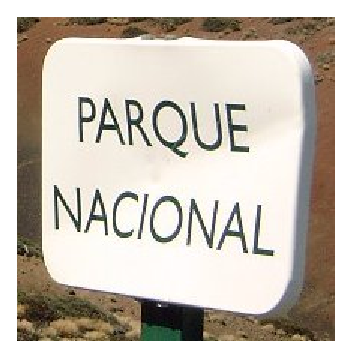
\includegraphics[scale=0.25]{parque-nacional}
    }
  }{label}
\end{pspicture}
\end{LTXexample}

\bigskip

\begin{LTXexample}[width=3.5cm]
\begin{pspicture}[showgrid=true](3,3)
  \pnode(0,0){A}
  \pnode(1.5,2){G}
  \pnode(3,1.5){B}
  \opttripole[beam](B)(G)(A){\rput[b](0,0){text}}{label}
\end{pspicture}
\end{LTXexample}

\medskip

\section{Fiber-Optical Objects}

\begin{description}
\paramitem{usefiberstyle}{<boolean>}{false}
\end{description}

Fiber-optical objects are automatically connected to the reference
nodes. The style of all fiber connections can be configured
independently (see Sec.~\ref{sec:fiberstyles}).

For some components it might me nice to highlight some
internals. If \Lkeyword{usefiberstyle} is enabled, for examples the
passing parts of the optical filter are drawn with the \styleshape{Fiber}
style. In the documentation this parameter is enabled to show the parts
which would be highlighted.

\subsection{Fiber}

\begin{BDef}
\fiberdipoledesc{optfiber}
\end{BDef}

\begin{description}
\paramitem{fiberloops}{<integer>}{3}
\paramitem{fiberloopradius}{<num>}{0.4}
\paramitem{fiberloopsep}{<num>}{0.3}
\end{description}
\medskip

\begin{LTXexample}[width=3.5cm]
\begin{pspicture}[showgrid=true](3,2)
  \optfiber[labeloffset=0.4](0,1)(3,1){SSMF}
\end{pspicture}
\end{LTXexample}

\medskip

\subsection{Amplifier}

\begin{BDef}
\fiberdipoledesc{optamp}
\end{BDef}

\begin{description}
\paramitem{optampsize}{<num>}{0.8}
\end{description}

\medskip

\begin{LTXexample}[width=3.5cm]
\begin{pspicture}[showgrid=true](3,2)
  \optamp(0,1)(3,1){EDFA}
\end{pspicture}
\end{LTXexample}

\medskip

\subsection{Mach-Zehnder Modulator}

\begin{BDef}
\fiberdipoledesc{optmzm}
\end{BDef}

\begin{description}
\paramitem{optmzmsize}{<num>}{0.8}
\end{description}

\medskip

\begin{LTXexample}[width=3.5cm]
\begin{pspicture}[showgrid=true](3,2)
  \optmzm(0,1)(3,1){MZM}
\end{pspicture}
\end{LTXexample}

\medskip

\subsection{Filter}

\begin{BDef}
\fiberdipoledesc{optfilter}
\end{BDef}

\begin{description}
\paramitem{filtersize}{<num>}{0.8}
\paramitem{filtertype}{bandpass|bandstop}{bandpass}
\end{description}

\medskip

\begin{LTXexample}[width=3.5cm]
\begin{pspicture}[showgrid=true](3,2)
  \optfilter(0,1)(3,1){bandpass}
\end{pspicture}
\end{LTXexample}

\bigskip

\begin{LTXexample}[width=3.5cm]
\begin{pspicture}[showgrid=true](3,2)
  \optfilter[filtertype=bandstop](0,1)(3,1){bandstop}
\end{pspicture}
\end{LTXexample}

\medskip

\subsection{Polarization Controller}

\begin{BDef}
\fiberdipoledesc{polcontrol}
\end{BDef}

\begin{description}
\paramitem{polcontrolsize}{<num>}{0.15}
\end{description}

\medskip

\begin{LTXexample}[width=3.5cm]
\begin{pspicture}[showgrid=true](3,2)
  \polcontrol(0,1)(3,1){PC}
\end{pspicture}
\end{LTXexample}

\medskip

\subsection{Isolator}

\begin{BDef}
\fiberdipoledesc{optisolator}
\end{BDef}

\begin{description}
\paramitem{isolatorsize}{<num>}{0.6}
\end{description}

\medskip

\begin{LTXexample}[width=3.5cm]
\begin{pspicture}[showgrid=true](3,2)
  \optisolator(0,1)(3,1){}
\end{pspicture}
\end{LTXexample}

\medskip

\subsection{Optical Switch}

\begin{BDef}
\fiberdipoledesc{optswitch}
\end{BDef}

\begin{description}
\paramitem{switchsize}{<num>}{0.8}
\paramitem{switchstyle}{opened|closed}{opened}
\end{description}

\medskip

\begin{LTXexample}[width=3.5cm]
\begin{pspicture}[showgrid=true](3,2)
  \optswitch(0,1)(3,1){Opened switch}
\end{pspicture}
\end{LTXexample}

\medskip

\begin{LTXexample}[width=3.5cm]
\begin{pspicture}[showgrid=true](3,2)
  \optswitch[switchstyle=closed](0,1)(3,1){Closed switch}
\end{pspicture}
\end{LTXexample}

\medskip

\subsection{Fiber Delay Line}

\begin{BDef}
\fiberdipoledesc{fiberdelayline}
\end{BDef}

\begin{description}
  \paramitem{fdlsize}{<num>}{0.6}
\end{description}

\medskip

\begin{LTXexample}[width=3.5cm]
\begin{pspicture}[showgrid=true](3,2)
  \fiberdelayline(0,1)(3,1){Delay line}
\end{pspicture}
\end{LTXexample}

\medskip


\subsection{Fiber Polarizer}

\begin{BDef}
\fiberdipoledesc{optfiberpolarizer}
\end{BDef}

\begin{description}
  \paramitem{fiberpolsize}{<num>}{0.6}
\end{description}

\medskip

\begin{LTXexample}[width=3.5cm]
\begin{pspicture}[showgrid=true](3,2)
  \optfiberpolarizer(0,1)(3,1){polarizer}
\end{pspicture}
\end{LTXexample}

\medskip

\subsection{Fiber Collimator}

\begin{BDef}
\Lcs{fibercollimator}\nodedescin\OptArg*{\nodedesc{A}}\OptArg*{\nodedesc{B}}\nodedescout\Largb{label}%
\end{BDef}

\begin{description}
\paramitem{fibercolsize}{<num>}{0.3}
\end{description}

The connection type for the fiber collimator is fixed
to \Lkeyword{conn=o-f}. The component can be use with two, three or
four nodes. With more than two points, the fiber is drawn as a
\Lcs{psbezier} curve. In the case of three nodes, the middle one is used
twice. Positioning parameters can still be used to shift the component
between the first two nodes.

\medskip

\begin{LTXexample}[width=3.5cm]
\begin{pspicture}[showgrid=true](3,2)
   \fibercollimator(0.5,1)(2.5,1){FC}
\end{pspicture}
\end{LTXexample}

\medskip

\begin{LTXexample}[width=3.5cm]
\begin{pspicture}[showgrid=true](3,2)
   \fibercollimator(0,1)(2,1)(3,2){FC}
\end{pspicture}
\end{LTXexample}

\medskip

\begin{LTXexample}[width=3.5cm]
\begin{pspicture}[showgrid=true](3,2)
   \fibercollimator(0.5,1)(2.5,1)(2.5,2){FC}
\end{pspicture}
\end{LTXexample}

\medskip

\begin{LTXexample}[width=3.5cm]
\begin{pspicture}[showgrid=true](3,2)
   \fibercollimator[position=0.2](0.5,1)(2.5,1)(2.5,2)(0.5,2){FC}
\end{pspicture}
\end{LTXexample}

\medskip

\subsection{Coupler}\label{sec:coupler}
\begin{description}
\paramitem{couplersize}{<num>}{0.2}
\paramitem{couplersep}{<num>}{0.1}
\paramitem{couplertype}{none|elliptic}{elliptic}
\paramitem{align}{top|bottom|center}{center}
\end{description}
\subsubsection{\texorpdfstring{$2\times 2$}{2x2} Coupler}

\medskip 

\begin{LTXexample}[width=3.5cm]
\begin{pspicture}[showgrid=true](3,2)
  \optcoupler(0.5,2)(0,0.5)(3,1.5)(2.5,0){Coupler}
\end{pspicture}
\end{LTXexample}

\bigskip

\begin{LTXexample}[width=3.5cm]
\begin{pspicture}[showgrid=true](3,2)
  \optcoupler[align=top](0.5,2)(0,0.5)(3,1.5)(2.5,0){Coupler}
\end{pspicture}
\end{LTXexample}

\bigskip

\begin{LTXexample}[width=3.5cm]
\begin{pspicture}[showgrid=true](3,2)
  \optcoupler[align=bottom, couplertype=none](0.5,2)(0,0.5)(3,1.5)(2.5,0){Coupler}
\end{pspicture}
\end{LTXexample}

\medskip

\subsubsection{WDM Coupler}

\medskip

\begin{LTXexample}[width=3.5cm]
\begin{pspicture}[showgrid=true](3,2)
  \wdmcoupler[labeloffset=0.5](0,1.5)(0,0.5)(3,1){WDM}
\end{pspicture}
\end{LTXexample}

\medskip

\subsubsection{WDM Splitter}
\begin{LTXexample}[width=3.5cm]
\begin{pspicture}[showgrid=true](3,2)
  \newpsstyle{FiberOut2}{style=Fiber, arrows=->}
  \wdmsplitter[align=top, labeloffset=0.5](0,1.5)(3,1.5)(3,0.5){}
\end{pspicture}
\end{LTXexample}

\medskip

\subsection{Fiber Styles}\label{sec:fiberstyles}

\begin{description}
\styleitem{Fiber}{<psstyle>}%{linecolor=red}
\styleitem{FiberIn}{<psstyle>}%{style=Fiber}
\styleitem{FiberIn1}{<psstyle>}%{style=FiberIn}
\styleitem{FiberIn2}{<psstyle>}%{style=FiberIn}
\styleitem{FiberOut}{<psstyle>}%{style=Fiber}
\styleitem{FiberOut1}{<psstyle>}%{style=FiberOut}
\styleitem{FiberOut2}{<psstyle>}%{style=FiberOut}
\end{description}

All these psstyles control the appearence of the fiber parts before and
after each object. The styles can be redefined with \Lcs{newpsstyle} or
changed with \Lcs{addtopsstyle}.  For optical systems it is not possible
to define a unique input and a unique output as most components can be
used bidirectionally. Therefore, I refer to the input as the connections
on the left of the object and to the output the ones on the right side.

The basic style is \styleshape{Fiber} which is the parent of all other
styles. \styleshape{FiberIn} inherits from \styleshape{Fiber} and defines
the style of the input fiber. Analogously \styleshape{FiberOut} controls
the style of the output fiber. If you want to change the input and
output fiber styles you should use \nxLcs{addtopsstyle} as then the
inheritance from the parent style \styleshape{Fiber} remains.

The other psstyles are used only by the various fiber couplers
(\Lcs{optcoupler}, \Lcs{wdmcoupler} and
\Lcs{wdmsplitter}). \styleshape{FiberIn1} affects the upper input fiber,
\styleshape{FiberIn2} the lower input fiber, \styleshape{FiberOut1} the
upper output fiber and \styleshape{FiberOut2} the lower output fiber. If
the object has only one input (e.g. \Lcs{wdmsplitter}),
\styleshape{FiberIn} is used. All fiber connections are drawn as
\Lcs{pccurve} which means that also the curvature and the input and
output angles of each connection can be changed as you will see in a
following code example.

\medskip

\begin{LTXexample}[width=3.5cm]
\begin{pspicture}[showgrid=true](3,3)
   \addtopsstyle{FiberIn}{ArrowInside=->, arrowscale=1.2}
   \addtopsstyle{FiberOut2}{linecolor=blue}
   \optcoupler(0,2.5)(0,0.5)(3,2.5)(3,0.5){50~\%}
\end{pspicture}
\end{LTXexample}

\medskip

In addition to the psstyles there exist
corresponding \Lkeyword{newFiber\ldots} and \Lkeyword{addtoFiber\ldots}
parameter keys for each of them.

\medskip

\begin{lstlisting}
\psset{addtoFiberIn={arrows=->, arrowscale=1.3}}
\end{lstlisting}

\medskip

\noindent is equivalent to 

\medskip

\begin{lstlisting}
\addtopsstyle{FiberIn}{arrows=->, arrowscale=1.3}
\end{lstlisting}

\medskip

\noindent Accordingly \Lkeyword{newFiberIn} corresponds to \Lcs{newpsstyle\{FiberIn\}\{\ldots\}}.

At first glance these keys make no sense. The reason why I
introduced them was to be able to define special couplers with
\Lcs{newpsobject}. This is only possible if all modifications can be
expressed as parameter keys. Consider for example a WDM splitter which
only couples out a certain spectral range of the input and you want to
mark the output with an arrow:

\medskip

\begin{LTXexample}[width=3.5cm]
\begin{pspicture}[showgrid=true](3,2)
   \newpsobject{mywdmsplitter}{wdmsplitter}{addtoFiberOut1={arrows=->, arrowscale=1.3, linecolor=blue}, labelangle=180, align=bottom}
   \mywdmsplitter(0,0.5)(3,1.5)(3,0.5){blue band}
\end{pspicture}
\end{LTXexample}

\medskip

Or if you need a coupler with a particular input angle you can do it be extending the appropriate fiber style:

\medskip

\begin{LTXexample}[width=3.5cm]
\begin{pspicture}[showgrid=true](3,2)
   \newpsobject{mycoupler}{optcoupler}{addtoFiberIn2={angleA=90}, align=top}
   \mycoupler(0.5,1.5)(0.5,0.5)(2.5,1.5)(2.5,0.5){}
\end{pspicture}
\end{LTXexample}

\medskip

\section{Connecting Objects}\label{sec:connecting}

\subsection{Drawing beams}\label{sec:drawbeam}
\begin{BDef}
  \Lcs{drawbeam}\OptArgs\Largb{Obj$_1$}\Largb{Obj$_2$}\ldots\Largb{Obj$_N$}
\end{BDef}
\begin{BDef}
  \Lcs{drawwidebeam}\OptArgs\Largb{Obj$_1$}\Largb{Obj$_2$}\ldots\Largb{Obj$_N$}
\end{BDef}

The package provides two macros for connecting objects with beams. Most
parameters are valid for both, those which are specifiy for wide beams are shown
in the next section. 

\subsubsection{Accessing objects}

The objects (specified as Obj$_1$, Obj$_2$, \ldots Obj$_N$ in the macro
definitions above) can be either components or PSTricks nodes. To distinguish
between named nodes and components, the node content must be enclosed in
parenthesis within the brackets. Components can be assigned a name explicitely
using \Lkeyword{compname} parameter, or they get a number in ascending order by
their definition in the code.

\begin{LTXexample}[width=4cm]
\begin{pspicture}(4,2)
  \pnode(0,1){A}\pnode(2,1){B}
  \optbox[endbox, labeloffset=0](A)(B){1}
  % connect a node with an object by its internal number
  \drawbeam{(A)}{1}
\end{pspicture}
\end{LTXexample}

\bigskip

\begin{LTXexample}[width=4cm]
\begin{pspicture}(4,2)
  \pnode(0,1){A}\pnode(2,1){B}
  \optbox[endbox, labeloffset=0, compname=obj](A)(B){obj}
  % connect a node with an object by its compname
  \drawbeam{(0,1)}{obj}
\end{pspicture}
\end{LTXexample}

\bigskip

The components which have an explicite name also increase the internal
counter, so that removing the \nxLkeyword{compname} from an intermediate
component does not affect the numbering of the following ones.

\medskip

\begin{LTXexample}[width=4cm]
\begin{pspicture}(4,3)
  \pnode(0,1){A}\pnode(2,1){B}
  \pnode(0,2){C}\pnode(2,2){D}
  \optbox[endbox, labeloffset=0, compname=obj](A)(B){obj}
  \optbox[endbox, labeloffset=0](C)(D){2}
  % connect a node with an object by its compname
  \drawbeam{(A)}{2}
\end{pspicture}
\end{LTXexample}

\medskip

\subsubsection{Internal component structure}

In order to understand properly how the automatic beam drawing actually works,
it is necessary to describe in more detail the internal component structure.

Every component type consists internally of interfaces which are defined by a
node on the optical axis, a plane vector or a curvature radius, and by its
optical characteristic (reflective or transmittive). The interface nodes can be
visualized for each component type with the \Lkeyword{showifcnodes}
parameter. 

\medskip

\begin{LTXexample}[width=4cm]
\begin{pspicture}(4,3)
  \psset{showifcnodes}
  \optbox(0,2.5)(4,2.5){}
  \doveprism(0,1.5)(4,1.5){}
  \lens(0,0.5)(4,0.5){}
  \mirror(0,0.5)(3.5,0.5)(3.5,3){}
\end{pspicture}
\end{LTXexample}

\bigskip

\nxLcs{draw*beam} calculates the distance between the interface nodes of two
objects and connects the two nearest

\medskip

\begin{LTXexample}[width=4cm]
\begin{pspicture}(-2,-2)(2,2)
  \psset{optboxwidth=0.6, optboxheight=0.5, labeloffset=0}
  \multido{\i=0+60,\ii=1+1}{6}{%
    \pnode(1.75;\i){A}
    \optbox([Xnodesep=-1]A)([Xnodesep=1]A){\ii}
  }
  \optbox[compname=ref](-1,0)(1,0){ref}
  \addtopsstyle{Beam}{arrows=->}
  \multido{\i=1+1}{6}{\drawbeam{ref}{\i}}
\end{pspicture}
\end{LTXexample}

\parampar{startpos}

This is the start position of the beam at the first interface. Can be
any code which evaluates in Postscript to one or two numbers. If is only
one number then the $x$-coordinate is set to \texttt{0}.

\begin{LTXexample}[width=5cm]
\begin{pspicture}(5,5)
  \pnode(1.5,0.5){A}\pnode(4.5,0.5){B}\pnode(3.5,4.5){C} 
  \optbox[endbox](B)(A){}
  \mirror[mirrorradius=4](A)(B)(C){} 
  \mirror[mirrortype=extended](B)(C)(B){} 
  \drawbeam[addtoBeam={linecolor=red},
              startpos=-0.2]{1}{2}{3}
  \drawbeam[addtoBeam={linecolor=blue},
              startpos=0]{1}{2}{3}
  \drawbeam[addtoBeam={linecolor=green},
              startpos=0.2]{1}{2}{3}
\end{pspicture}
\end{LTXexample}

\medskip

\parampar{startvec} This is the start vector of the beam.

\begin{LTXexample}[width=5cm]
\begin{pspicture}(5,5)
  \pnode(1.5,0.5){A}\pnode(4.5,0.5){B}\pnode(3.5,4.5){C} 
  \optbox[endbox](B)(A){}
  \mirror[mirrorradius=2](A)(B)(C){} 
  \mirror[mirrortype=extended](B)(C)(B){} 
  \drawbeam[addtoBeam={linecolor=red},
              startvec=0.05]{1}{2}{3}
  \drawbeam[addtoBeam={linecolor=blue},
              startvec=0]{1}{2}{3}
  \drawbeam[addtoBeam={linecolor=green},
              startvec=-0.05]{1}{2}{3}
\end{pspicture}
\end{LTXexample}

\medskip

\parampar{startvecabs}

\parampar{connectplanes}

\parampar{n}

\parampar{beaminside}

\parampar{beaminsidelast}

\parampar{beaminsidefirst}

\subsection{Drawing wide beams}\label{sec:drawwidebeam}

\parampar{beamwidth}

\parampar{beamdiv}

\subsection{Drawing fibers}\label{sec:drawfiber}
\begin{BDef}
  \Lcs{drawfiber}\OptArgs\Largb{$C_1$}\Largb{$C_2$}
\end{BDef}

\begin{LTXexample}[width=4cm]
\begin{pspicture}[showgrid=true](2.8,3)
\pnode(0.3,0){A}
\pnode(2.3,0){B}
\pnode(0.3,3){C}
\pnode(2.3,3){D}
\optcoupler[abspos=0.5, nofiber](A)(B)(C)(D){}
\optbox[abspos=2, optboxwidth=0.5,optboxheight=0.5](C|A)(C){}
\optfiber[nofiber](D)(C){}
\optamp[nofiber, abspos=2](D|A)(D){}
\drawfiber[angleA=0, ArrowInside=->]{(A)}{1}
\drawfiber[angleB=180, arrows=->]{1}{(B)}
\drawfiber{1}{2}
\drawfiber{2}{3}
\drawfiber{3}{4}
\drawfiber{4}{1}
\end{pspicture}
\end{LTXexample}

\subsection{Custom beams}\label{sec:custombeam}
\begin{BDef}
  \Lcs{custombeam}\OptArgs\lcb\nxLcs{draw*beam}\rcb
\end{BDef}

\parampar{startinside}

\parampar{stopinside}

% \begin{description}
% \paramitem{conn}{<conn definition>}{-}
% \item[\param{fiber}:] alias for \Lkeyword{conn=f-f}
% \item[\param{beam}:] alias for \Lkeyword{conn=o-i}
% \paramitem{connjoin}{<int>}{1}
% \end{description}

% \noindent Simple experimental setups with a few objects can usually be
% realized by defining some nodes, arranging the object in between and
% drawing the beams at the end. If, however, objects with changed internal
% optical path (all the prisms) or without visible internal beam (optical
% diode) are involved, this simple method is not applicable anymore.

% For this case several different possibilities of connecting objects are
% available: \Lkeyword{conn} specifies the kind of connections in front of and
% behind the object. Its syntax is analogous to the PSTricks
% \Lkeyword{arrows} parameter. By default it is set to \paramvalue{-} and no
% connections are drawn. Tab.~\ref{tab:conn} lists all possible values and
% their scope for the \paramvalue{<conn definition>}.

% \begin{table}\centering
% \addtolength{\extrarowheight}{1.5mm}
% \begin{tabularx}{0.9\textwidth}{TXl}
%   \toprule
%   \multicolumn{1}{l}{conn style} & description & scope\\
%   \midrule
%   i & Draw beam from the first reference node to its assigned outer node 
%       and then through all internal nodes and end at the other 
%       outer node. & \multirow{3}{*}{optexp objects}\\
%   o & Draw beam from the first reference node to its assigned outer node.  & \\
%   f & Draw fiber from the first reference node to its assigned outer node. & \\
%   \midrule
%   a & Left outer node & \multirow{4}{*}{\Lcs{drawbeam} macro}\\
%   A & Connect left outer node to all internal nodes and then to the right outer node & \\
%   b & Right outer node & \\
%   B & Connect right outer node to all internal nodes and then to the left outer node & \\
%   \bottomrule
% \end{tabularx}
% \caption{All possible values for the \paramvalue{<conn definition>}, their detailed description and scope.}\label{tab:conn}
% \end{table}

% The first letter (before the dash) in the \paramvalue{<conn definition>}
% refers to which object node the first reference node should be connected
% to, the second letter (after the dash) affects the connection from the
% object to the second reference node. Tab.~\ref{tab:conn} lists all
% possibilities for \Lkeyword{conn} within an object: \paramvalue{f} draws
% a fiber connection and \paramvalue{o} a beam connection to the
% appropriate outer node. \paramvalue{i} draws a beam connection to the
% appropriate outer node and then through all internal nodes and end at
% the other outer node. The boolean parameter \Lkeyword{beam} is an alias
% for \Lkeyword{conn=o-i}. The beam style is controlled by the
% psstyle \styleshape{Beam} which can be changed
% using \Lcs{newpsstyle} and \Lcs{addtopsstyle}.

% All fiber-optical units define \Lkeyword{conn=f-f} which means that
% input and output connections are \paramvalue{f}ibers. The boolean
% parameter \Lkeyword{fiber} is an alias for \Lkeyword{conn=f-f}. The
% fiber connection style can be changed by adapting the \styleshape{Fiber*}
% styles (see Sec.~\ref{sec:fiberstyles}).

% The way how to really use this kind of connections should become more
% clear after looking at the following examples in this section.

% \medskip

% \begin{LTXexample}[width=4.5cm]
% \begin{pspicture}[showgrid=true](4,5)
%   \addtopsstyle{Beam}{arrows=->, arrowscale=1.5}
%   \psset{labeloffset=0}
%   \doveprism[conn=o-](0,4.5)(4,4.5){\texttt{o-}}
%   \doveprism[conn=i-](0,3.5)(4,3.5){\texttt{i-}}
%   \doveprism[conn=-o](0,2.5)(4,2.5){\texttt{-o}}
%   \doveprism[conn=-i](0,1.5)(4,1.5){\texttt{-i}}
%   \optbox[conn=-f](0,0.5)(4,0.5){\texttt{-f}}
% \end{pspicture}
% \end{LTXexample}

% \medskip 

% The following example shows how this \Lkeyword{conn} parameter can be used in some kinds
% of experimental setups using objects with changed internal optical path (here a
% penta prism). Instead of drawing the beam at the end with a \Lcs{psline},
% the beams are created at definition time of the respective object.

% \begin{LTXexampleFloat}
% \begin{LTXexample}[width=4.5cm]
% \begin{pspicture}[showgrid=true](4,5)
%    \pnode(1,1){A}\pnode(1,4){G}\pnode(3,4){B}
%    \optbox[endbox, labelref=relative, labeloffset=0, optboxwidth=1](G)(A){Laser}
%    \lens[lens=0.5 0.5 0.5, abspos=0.3](A)(G){}
%    \pinhole[abspos=0.5](A)(G){}
%    \lens[lens=2, abspos=0.8](A)(G){}
%    \lens[abspos=2, labelangle=180](A)(G){L}
%    \optplate[abspos=1.5, labeloffset=1](A)(G){SLM}
%    \lens[abspos=1](G)(B){L}
%    \optbox[endbox, labeloffset=0, optboxwidth=1](G)(B){CCD}
%    \pentaprism[beam, labeloffset=1](A)(G)(B){PP}
% \end{pspicture}
% \end{LTXexample}
% \caption{Code example on how to use the \Lkeyword{conn} parameter in experimental setups.}\label{lst:conn}
% \end{LTXexampleFloat}

% \begin{BDef}
% \Lcs{drawbeam}\OptArg{conn=\ldots}\Largb{<from>}\Largb{<to>}
% \end{BDef}
% This method works unless objects without internal beams (e.g. an optical
% diode, Sec.~\ref{sec:optdiode}) or with internal reflections (e.g. a
% Dove prism, Sec.~\ref{sec:doveprism}) are used in the straight light
% paths of the setup. One possibility would be to create additional nodes,
% but this may be not very comfortable. Therefore, \LPack{pst-optexp}
% provides a macro \Lcs{drawbeam} which connects a named object
% (Sec.~\ref{sec:namedobj}) to another named object or a node.

% \medskip

% \noindent If \paramvalue{<from>} or \paramvalue{<to>} is a node, it must be written
% including the round braces. The call

% \medskip

% \begin{lstlisting}
% \drawbeam{Obj}{(1;45)}
% \end{lstlisting}

% \medskip\noindent connects the named object \nodename{Obj} to the node.

% The type of beam connection which \Lcs{drawbeam} draws is again
% controlled by the parameter \Lkeyword{conn}. Almost every optical
% object does not have distinguished inputs and outputs and can be used in
% either directions. Therefore, it does not make sense to speak about
% `input` and `output` when referring to the object nodes, but rather
% about node A (\nodename{left outer node}) and node B (\nodename{right outer
%   node}). Consequently, the two letters of parameter \Lkeyword{conn}
% can take the values \paramvalue{a}, \paramvalue{A}, \paramvalue{b}
% or \paramvalue{B} when used together with \Lcs{drawbeam}. The detailed
% descriptions of the individual possibilities are listed in
% Tab.~\ref{tab:conn}. The letter before the dash in \Lkeyword{conn}
% refers to the \paramvalue{<from>} object, the other one to
% the \paramvalue{<to>} object. Again, the next examples should clearify
% how to apply the \Lcs{drawbeam} macro together with the
% different \Lkeyword{conn} settings.

% \begin{LTXexampleFloat}
%   \begin{LTXexample}[width=4.5cm]
%     \begin{pspicture}[showgrid=true](4,6) \psset{labeloffset=0.6}
%       \addtopsstyle{Beam}{arrows=->, arrowscale=1.5}
%       \doveprism[compname=Dove1](0,0.8)(3,0.8){Dove1}
%       \drawbeam[conn=b-]{Dove1}{(3,0.8)}
%       \doveprism[compname=Dove2](0,2.3)(3,2.3){Dove2}
%       \drawbeam[conn=B-]{Dove2}{(3,2.3)}
%       \doveprism[compname=Dove3](0,3.8)(3,3.8){Dove3}
%       \drawbeam[conn=-a]{(0,3.8)}{Dove3}
%       \doveprism[compname=Dove4](0,5.3)(3,5.3){Dove4}
%       \drawbeam[conn=-A]{(0,5.3)}{Dove4}
%     \end{pspicture}
%   \end{LTXexample}
% \end{LTXexampleFloat}

% With the help of the \Lcs{drawbeam} macro we can adapt
% Listing~\ref{lst:conn} to use an optical diode before the beam clearing
% and connect it to the other components. In order to illustrate the beams
% that are drawn by the different mechanisms, they are colorcoded in the
% resulting Listing~\ref{lst:conn2}: \emph{green} is the direct connecting
% of the optical diode, \emph{red} is the \nxLcs{drawbeam} connection and
% \emph{blue} the direct connecting of the penta prism.

% \begin{LTXexampleFloat}
% \begin{LTXexample}[width=4.5cm]
% \begin{pspicture}[showgrid=true](4,6)
%    \pnode(1,1){A}\pnode(1,5){G}\pnode(3,5){B}
%    \optbox[endbox, labelref=relative, labeloffset=0, optboxwidth=1](G)(A){Laser}
%    \lens[lens=0.5 0.5 0.5, abspos=1.5](A)(G){}
%    \pinhole[abspos=1.7](A)(G){}
%    \lens[lens=2, abspos=2](A)(G){}
%    \lens[abspos=3, labelangle=180](A)(G){L}
%    \optplate[abspos=2.5, labeloffset=1](A)(G){SLM}
%    \lens[abspos=1](G)(B){L}
%    \optbox[endbox, labeloffset=0, optboxwidth=1](G)(B){CCD}
%    \optdiode[abspos=0.8, conn=o-, compname=OD](A)(G){OD}
%    \addtopsstyle{Beam}{linecolor=blue}
%    \pentaprism[conn=-i, labeloffset=1, compname=PP](A)(G)(B){PP}
%    \addtopsstyle{Beam}{linecolor=red}
%    \drawbeam[conn=b-a]{OD}{PP}
% \end{pspicture}
% \end{LTXexample}
% \caption{More soffisticated code example which employs both connecting
%   methods. The beam connections are colorcoded: \emph{green} is the
%   direct connecting of the optical diode, \emph{red} is the
%   \Lcs{drawbeam} connection and \emph{blue} the direct connecting of the
%   penta prism.}\label{lst:conn2}
% \end{LTXexampleFloat}


\section{Defining New Objects}

\subsection{Customized Versions of Existing Macros}

The easiest way to define your own components is to use the
\Lcs{newpsobject} macro. With this you can define a new component using
predefined objects with a set of options. These options serve only as
default values and can be overridden when calling the macro. The
following examples defines a new object \nxLcs{sbn} for the special crystal
used in Sec.~\ref{sec:crystal}.

\medskip

\begin{LTXexample}[width=3.5cm]
\newpsobject{sbn}{crystal}{voltage, lamp, labelangle=45, labeloffset=1.2, fillstyle=solid, fillcolor=yellow!90!black}
\begin{pspicture}[showgrid=true](3,2) 
   \sbn(0,1)(3,1){SBN:Ce}
   \psline[style=Beam](0,1)(3,1)
\end{pspicture}
\end{LTXexample}

\medskip

\begin{LTXexample}[width=3.5cm]
\newpsobject{pumpcoupler}{wdmcoupler}{align=top, labelangle=180, labeloffset=0.5,addtoFiberIn2={ArrowInside=->, arrowscale=2}}
\begin{pspicture}[showgrid=true](3,2) 
   \pumpcoupler(0,1)(0,0)(3,1){Pumpcoupler}
\end{pspicture}
\end{LTXexample}

\medskip

Or if you need more than one type of lenses several times in your setup
it is very cumbersome to specify all parameters every time.

\medskip

\begin{LTXexample}[width=5.5cm]
\newpsobject{MOLensIn}{lens}{lens=0.5 0.5 0.5}
\newpsobject{MOLensOut}{lens}{lens=1.5 1.5 1.5}
\begin{pspicture}[showgrid=true](5,2) 
   \pnode(0,1){A}\pnode(5,1){B}
   \psset{n=1}
   \MOLensIn[abspos=0.5](A)(B){}
   \MOLensOut[abspos=1](A)(B){}
   \MOLensOut[abspos=4](A)(B){}
   \MOLensIn[abspos=4.5](A)(B){}
   \custombeam{%
     \drawwidebeam[beamwidth=0.1]{(A)}{1}
     \drawwidebeam[beamdiv=1]{1}{2}
   }
\end{pspicture}
\end{LTXexample}
\medskip

\subsection{Defining New Objects}\label{sec:newobj}

Since version 1.2 \nxLPack{pst-optexp} provides some high-level macros to
allow very convenient definition of completely new components. The macro
\Lcs{newOptexpDipole} generates all organizing code for a new free-ray
component. All you have to do is to define a new `drawing' macro
\nxLcs{mycomponent@iii} which contains all drawing code. Analogously
\Lcs{newOptexpDipoleNolabel} defines a new free-ray object without label
(like \Lcs{polarization}) and \Lcs{newOptexpTripole} defines a new
reflective component. 

New fiber-optical components can be defined using
\Lcs{newOptexpFiberDipole}. This macro differs from its free-ray
analogous only in that it presets \Lkeyword{fiber} and hence directly
connects the component with its reference nodes. The first node in the
parameter list gets connected with a node \nodename{tempNode@A@}, the
second node with a node \nodename{tempNode@B@}. These two internal
nodes are preset to \paramvalue{(0,0)} and can be overwritten within the
drawing macro.

The syntax of the macros is
\begin{lstlisting}
\newOptexpDipole[fixed options]{name}{default options}
\newOptexpDipoleNolabel[fixed options]{name}{default options}
\newOptexpTripole[fixed options]{name}{default options}
\newOptexpFiberDipole[fixed options]{name}{default options}
\end{lstlisting}
The \texttt{default options} are simply a list of PSTricks parameters
which are taken as defaults for the new component. The optional argument
allows setting of parameters which cannot be overridden later.

This is illustrate a bit more in the next code snippet, which also shows
how the coordinate system is handled within the \nxLcs{mycomponent@iii}
macro.

\medskip

\begin{LTXexample}[width=4.5cm]
\newOptexpTripole{mygrid}{subgriddiv=5, griddots=0, subgridwidth=\pslinewidth, gridwidth=2\pslinewidth}
\makeatletter
\def\mygrid@iii{% put here all PSTricks drawing code
  \psgrid(-1,0)(1,1)
}%
\makeatother
\begin{pspicture}[showgrid=true](4,4) 
   \pnode(0,1){A}\pnode(2,2){G}\pnode(3,0){B}
   \mygrid[gridcolor=red,labeloffset=1.5](A)(G)(B){myGrid}
   \psline[style=Beam](A)(G)(B)
\end{pspicture}
\end{LTXexample}
\medskip

The default position of the label reference point is (0,0). If you want
to change this, you have to define a new pnode named
\nodename{tempNode@Label} in the \nxLcs{mycomponent@iii} macro.

If you create a new component, please send it to me then I can
incorporate this in a new released version.

\newpage

\section{Examples}
\begin{LTXexample}[pos=t,vsep=8mm]
\begin{pspicture}(10,2)
\psset{optboxwidth=1}\addtopsstyle{Beam}{linewidth=2\pslinewidth}
\pnode(1,1){Start}\pnode(9,1){CCD}\optbox[endbox, labeloffset=0](CCD)(Start){Laser}
\optbox[endbox,labeloffset=0,beam](Start)(CCD){CCD}
\polarization[poltype=perp,abspos=0.5](Start)(CCD)
\optretplate[abspos=1](Start)(CCD){$\nicefrac{\lambda}{2}$}
\lens[lens=0.4 0.4 0.5,abspos=2](Start)(CCD){$L_1$}\lens[abspos=4](Start)(CCD){$L_2$}
\optplate[abspos=6,platelinewidth=3\pslinewidth](Start)(CCD){SLM}
\optplate[abspos=6.5,labelangle=180](Start)(CCD){PF}
\polarization[abspos=6.7](Start)(CCD)\lens[abspos=7](Start)(CCD){$L_3$}
\end{pspicture}
\end{LTXexample}

\vspace{\fill}

\begin{LTXexample}[pos=t,vsep=8mm]
\begin{pspicture}(-4,-1)(3,3)
\addtopsstyle{Beam}{linewidth=2\pslinewidth, linecolor=red!90!black}
\psset{labeloffset=0.5}
\pnode(-2,0){LaserOut}\pnode(0,0){Grat}
\pnode(4;45){Out}\pnode(2.5;67.5){Mvar}
\optbox[optboxwidth=2,labeloffset=0, endbox](Grat)(LaserOut){diode laser}
%\mirror[variable,conn=o-](Grid)(Mvar)(Grid){M$_\mathrm{var}$}
\optgrid[beam](LaserOut)(Grat)(Out){grating}
\optretplate[position=0.3,labeloffset=0.8]%
  (LaserOut)(Grat){$\nicefrac{\lambda}{4}$}
\rput[l](-3,2){Littman setup}
\end{pspicture}
\end{LTXexample}

\begin{LTXexample}[pos=t, vsep=8mm]
\begin{pspicture}(8.5,1.6)
    \addtopsstyle{Beam}{linecolor=green!90!black}
    \pnode(1.6,1){Laser}\pnode(7.6,1){Diode}
    \optbox[endbox,labeloffset=0](Diode)(Laser){Laser}%
%    \optbox[abspos=4, optboxwidth=1, optboxheight=0.6, labeloffset=1, compname=PC, conn=o-, angle=-10, rotateref=l, refractiveindex=2.3](Laser)(Diode){Photonic Crystal}
%    \optdetector[dettype=diode, conn=o-](\OENodeOut{PC})(Diode|\OENodeOut{PC}){PD}
    \optbox[abspos=4, optboxwidth=1, optboxheight=0.6, labeloffset=1, compname=PC, angle=-10, rotateref=l, refractiveindex=2.3](Laser)(Diode){Photonic Crystal}
    \optdetector[dettype=diode](\OENodeOut{PC})(Diode|\OENodeOut{PC}){PD}
    \defShiftedNode(\OENodeIn{PC})(2;170){Angle1}
    \psline[linestyle=dashed](\OENodeIn{PC})(Angle1)
    \psarc{<->}(\OENodeIn{PC}){1.3}{330}{30}
    \psarc[arcsep=1pt]{<->}(\OENodeIn{PC}){2}{170}{180}
    \uput{2.1}[175](\OENodeIn{PC}){\small $\varphi$}
\end{pspicture}
\end{LTXexample}

\begin{LTXexample}[pos=t, vsep=8mm]
\begin{pspicture}(6.4,3.2)
\addtopsstyle{Fiber}{linecolor=red}
\pnode(2.3,2.3){Lin}\pnode([Xnodesep=0.5]Lin){Lout}
\pnode([Xnodesep=1.5]Lout){EAMout}
\pnode([Xnodesep=1.5]EAMout){Det}
\optbox[fiber, 
labeloffset=-0.2, endbox, compname=L, extnode=b](Lout)(Lin){%
    \psGauss[yunit=0.03,sigma=0.03]{-0.5}{0.5}}
\optbox[fiber, 
labeloffset=0, optboxwidth=1, compname=EAM, extnode=b](Lout)(EAMout){EAM}
\optfiber[labeloffset=0.3](EAMout)(Det){fibre}
\optdetector(EAMout)(Det){OSA}
\pnode([Xnodesep=-1,offset=-1]LExtNode){Osc}
\pnode(LExtNode|Osc){PSin}\pnode(EAMExtNode|Osc){PSout}
\oscillator[output=right](Osc){10\,GHz}{}
\phaseshifter[labeloffset=-0.7](PSin)(PSout){$\tau$}
\wire(LExtNode)(PSin)\wire(EAMExtNode)(PSout)
\end{pspicture}
\end{LTXexample}

\begin{LTXexample}[pos=t, vsep=8mm]
\begin{pspicture}(0.9,0.9)(10.4,5.9)
  \psset{arrowscale=1.5, arrowinset=0}
  \addtopsstyle{Fiber}{linewidth=2\pslinewidth}
  \pnode(2,5){PC1in}\pnode(4,5){PC1out}\pnode(6,5){PC2in}
  \pnode(8,5){PC2out}\pnode(2,2){CplSig}\pnode(5,2){CplIn}
  \pnode(2,1){CplOut}\pnode(10,4.5){Pump}\pnode(8,2){PumpSig}
  \optisolator[compshift=0.8, addtoFiberIn={angleA=180}, addtoFiberOut={angleB=180}, labelref=relative, labeloffset=0.6](CplSig)(PC1in){isolator}
  \polcontrol[addtoFiberIn={arrows=|-}](PC1in)(PC1out){}
  \optfiberpolarizer[labeloffset=0.6](PC1out)(PC2in){polarizer}
  \polcontrol[addtoFiberOut={arrows=-|}](PC2in)(PC2out){}
  \wdmsplitter[labeloffset=0.3, align=bottom, addtoFiberIn={arrows=|-}, addtoFiberOut1={arrows=->}, addtoFiberOut2={arrows=-|}](CplIn)(CplOut)(CplSig){95/5}
  \wdmcoupler[addtoFiberIn1={ArrowInside=->}, addtoFiberIn2={angleA=0}, addtoFiberOut={angleB=0,arrows=-|}, ncurv=0.9, align=bottom, compshift=0.8](Pump)(PC2out)(PumpSig){Pump}
  \optbox[endbox,labeloffset=0,labelref=relative]([offset=-0.1]Pump)(Pump){980~nm}
  \optfiber[fiberloops=2, labeloffset=0.4](CplIn)(PumpSig){Er$^+$-doped}
\end{pspicture}
\end{LTXexample}

\begin{LTXexample}[pos=t, vsep=8mm]
\makeatletter
\def\LCLV@nodes{%
  \newOptexpComp{ {-0.12 0} {0 1} trans {NewPlaneInt}
                  {0.15 0} {0 1} trans {NewPlaneInt} \psk@oe@n}%
}%
\def\LCLV@comp{%
  \psframe[fillstyle=solid,fillcolor=black,dimen=outer](-0.12,-0.5)(0,0.5)
  \psframe[fillstyle=solid,fillcolor=gray!50,dimen=outer](0,-0.5)(0.15,0.5)
}%
\makeatother
\begin{pspicture}(9,5)
\newOptexpDipole{LCLV}{}\psset{lens=1.2 0 1}
\pnode(2.4,1){BS1}\pnode([offset=3]BS1){M1}\pnode([Xnodesep=5.5]M1){PP}\pnode(PP|BS1){BS2}
\LCLV[position=0.2, compname=LCLV](BS1)(BS2){LCLV}\beamsplitter[compname=BS](BS2)(BS1)(M1){BS}
\optretplate(BS1)(M1){P}\mirror(BS1)(M1)(PP){M}\lens[position=0.2](M1)(PP){L}
\pinhole(M1)(PP){}\lens[position=0.2](PP)(M1){L}\pentaprism(M1)(PP)(BS2){PP}
\beamsplitter(PP)(BS2)(BS1){BS}\lens(BS2)(BS1){L}
\doveprism[compname=Dove,position=0.27](BS2)(BS1){D}
\addtopsstyle{Beam}{arrowscale=1.3, ArrowInside=-<}
\optbox[labeloffset=0, endbox](BS1)([Xnodesep=-1]BS1){Nd:YAG}
\drawbeam{LCLV}{BS}
\end{pspicture}
\end{LTXexample}

%\begin{LTXexample}[pos=t,vsep=8mm]
\begin{pspicture}(0,-0.4)(9,6)
  \addtopsstyle{Beam}{linewidth=2\pslinewidth}
  \pnode(1.5,5){Laser}\pnode(4,5){PBS}\pnode(6.5,5){PBS2}
  \pnode(6.5,5.7){piezo}\pnode(4,2){BSFwd}\pnode(6.5,2){BSBwd}
  \pnode(2,2){BS4f}\pnode(2,0.5){M4f3}\pnode(8,2){M4f1}
  \pnode(8,0.5){M4f2}\pnode(1,2){CCD}
  \psline[style=Beam](Laser)(PBS2)(piezo)(BSBwd)(M4f1)(M4f2)(M4f3)(BS4f)(CCD)
  \psline[style=Beam](PBS)(BSFwd)(BS4f)
  \psset{mirrorwidth=0.6, plateheight=0.7, outerheight=0.7, labeloffset=0.7, labelstyle=\scriptsize, lens=1.2 1.2 0.8, bssize=0.5} 
  \optbox[endbox,optboxwidth=1.5, optboxheight=0.7,labeloffset=0]%
     (PBS)(Laser){\parbox{1.5cm}{\centering Nd:YAG\\ 532\,nm}}
  \lens[lensheight=0.5, position=0.2](Laser)(PBS){MO}
  \pinhole[position=0.3,labelangle=180](Laser)(PBS){PH}
  \lens[position=0.5](Laser)(PBS){L}
  \optretplate[position=0.8](Laser)(PBS){$\nicefrac{\lambda}{2}$}
  \beamsplitter(Laser)(PBS)(BSFwd){PBS}
  \optretplate[position=0.4](PBS)(BSFwd){$\nicefrac{\lambda}{2}$}
  \polarization(PBS)(BSFwd)\polarization(PBS2)(BSBwd)
  \lens[position=0.8](PBS)(BSFwd){L}
  \optretplate(PBS)(PBS2){$\nicefrac{\lambda}{2}$}
  \beamsplitter(PBS)(PBS2)(piezo){PBS}
  \optretplate[abspos=0.5](PBS2)(piezo){$\nicefrac{\lambda}{4}$}
  \mirror[mirrortype=piezo,labelangle=90](PBS2)(piezo)(PBS2){PZ}
  \lens[position=0.8,labelangle=180](PBS2)(BSBwd){L}
  \crystal[crystalwidth=1, crystalheight=0.5, voltage, lamp, fillstyle=solid, fillcolor=yellow!90!black, labeloffset=0.8, beam](BSFwd)(BSBwd){SBN:Ce}
  \beamsplitter(PBS)(BSFwd)(BSBwd){BS}
  \beamsplitter[labelangle=-90](PBS2)(BSBwd)(BSFwd){BS}
  \mirror(BSBwd)(M4f1)(M4f2){M}\mirror(M4f1)(M4f2)(M4f3){M}
  \lens[labelangle=180](M4f2)(M4f3){L}\mirror(M4f2)(M4f3)(BS4f){M}
  \beamsplitter(M4f3)(BS4f)(CCD){BS}\optbox[endbox,labeloffset=0, optboxwidth=1](BS4f)(CCD){CCD}
  \lens[abspos=0.7](BS4f)(BSFwd){L}\lens[abspos=0.7](BSBwd)(M4f1){L}
\end{pspicture}
%\end{LTXexample}

\psset{unit=0.8cm,labelstyle=\footnotesize}
%\begin{LTXexample}[pos=t]
\begin{pspicture}(0.5,4)(13.2,10.5)
  \addtopsstyle{Fiber}{linecolor=red!90!black}\psset{usefiberstyle, optboxwidth=1}
  \pnode(2,10){LD}\pnode([Xnodesep=5.5]LD){CPLin1}
  \pnode([offset=-2]CPLin1){CPLin2}\pnode([Xnodesep=1.5]CPLin1){CPLout1}
  \pnode([Xnodesep=1.5]CPLin2){CPLout2}
  \optbox[endbox, labeloffset=0, fiber]([Xnodesep=0.1]LD)(LD){LD}
  \optmzm([Xnodesep=0.1]LD)([Xnodesep=1.5]LD){MZM}
  \optamp([Xnodesep=1.5]LD)([Xnodesep=2.5]LD){EDFA}
  \optfilter([Xnodesep=2.5]LD)([Xnodesep=3.5]LD){BPF}
  \optswitch([Xnodesep=3.5]LD)([Xnodesep=4.5]LD){SW}
  \polcontrol([Xnodesep=4.5]LD)(CPLin1){}
  \optcoupler[couplertype=none](CPLin1)(CPLin2)(CPLout1)(CPLout2){}
  \optamp(CPLout1)([Xnodesep=1.5]CPLout1){EDFA}
  \optfilter([Xnodesep=1.5]CPLout1)([Xnodesep=3]CPLout1){BPF}
%  \optbox[endbox, labeloffset=0, conn=f-f]([Xnodesep=3]CPLout1)([Xnodesep=3.1]CPLout1){RX}
  \pnode([Xnodesep=2]CPLout2){LoopRU}\pnode([offset=-3.5]LoopRU){LoopRL}
  \pnode([Xnodesep=-5]CPLin2){LoopLU}\pnode([offset=-3.5]LoopLU){LoopLL}
  \optamp(CPLout2)(LoopRU){EDFA}
  \psline[linearc=1,style=Fiber](LoopRU)([Xnodesep=1]LoopRU)([Xnodesep=1,offset=-2]LoopRU)
  \psline[linearc=1,style=Fiber]([Xnodesep=1,offset=1.5]LoopRL)%
                                ([Xnodesep=1]LoopRL)(LoopRL)
  \optfiber[labelalign=b, labeloffset=-1, position=0.8]([Xnodesep=-2]LoopRL)(LoopRL){\begin{tabular}{c}conventional\\fibre 89.8~km\end{tabular}}
  \optamp([Xnodesep=-2]LoopRL)([Xnodesep=-3]LoopRL){EDFA}
  \optfilter([Xnodesep=-3]LoopRL)([Xnodesep=-4.5]LoopRL){BPF}
  \optfiber[fiberloops=1, labeloffset=-1, labelalign=b]([Xnodesep=-7]LoopRL)([Xnodesep=-4.5]LoopRL){DCF 16.2~km}
  \optamp([Xnodesep=1.5]LoopLL)(LoopLL){EDFA}
  \psline[style=Fiber,linearc=1](LoopLL)([Xnodesep=-1]LoopLL)%
                                ([Xnodesep=-1,offset=3.5]LoopLL)(LoopLU)
  \optfilter(LoopLU)([Xnodesep=1.5]LoopLU){BPF}
  \optswitch([Xnodesep=1.5]LoopLU)([Xnodesep=3.5]LoopLU){SW}
  \polcontrol([Xnodesep=3.5]LoopLU)(CPLin2){}
\end{pspicture}
%\end{LTXexample}

\section{Requirements}

\LPack{pst-optexp} version 3.0 requires at least version 2.87 of
\LPack{pstricks-add}, \LPack{multido}, \LPack{pst-eucl}, \LPack{environ} and
\LaTeX. It does not work with plain \TeX.

\section{Todo}

\begin{itemize}
\item Automatic sizing of optboxes (like a \Lcs{psframebox}
\end{itemize}

\section{Acknowledgements}

I thank all the people of the PSTricks mailinglist for the continuous help, especially Herbert Vo�.


\printindex
\end{document}
